\documentclass{article}
\usepackage{spconf,amsmath,graphicx,color,hyperref}

\newcommand{\todo}[1]{
    \textcolor{red}{#1}
}

\title{HIPPOCAMPAL SEGMENTATION WITH A VERY SMALL ATLAS LIBRARY: THE MAGET
BRAIN ALGORITHM} 
\name{  Jon Pipitone$^{\star}$ Jason P. Lerch$^{\dagger}$ Miriam Friedel$^{\dagger}$ Aristotle Voineskos$^{\star}$
         Mallar Chakravarty$^{\star}$ }  

\address{$^{\star}$ Centre for Additions and Mental Health, Toronto ON, Canada \\
     $^{\dagger}$ Mouse Imaging Centre, ..., Toronto ON, Canada}

\usepackage{Sweave}
\begin{document}
\input{paper-concordance}
\maketitle       

\begin{abstract}
Neuroimaging research often relies on automated anatomical
segmentations of MR images of the brain. Current multi-atlased based
approaches provide accurate segmentations of brain images by
propagating region labels from manual delineations to unlabeled
images.  Unfortunately, these approaches often rely on a large number
of such manual segmentations which take time and significant expertise
to produce, neither of which may be readily available.  We present
an algorithm for the automatic segmentation of the hippocampus that
minimizes the number of atlases needed whilst still achieving nearly
the same accuracy as other multi-atlas approaches.  We perform
repeated random sub-sampling validation on the IBSR dataset to
validate our approach and find an average best case percent difference
to the multi-atlas approach of 1.9\%. {I STILL THINK THAT HIS SENTENCE NEEDS TO BE CLEARER; BREAK THIS OUT INTO TWO SENTENCES - OR MORE- WHERE FIRST YOU TALK ABOUT THE VALIDATION APPROACH, INCLUDING THE DIFFERENT METHODOLOGIES.  IN A SECOND SENTENCE YOU SHOULD DISCUSS THE RESULTS.  ALSO I THINK WE NEED SOME EMPHASIS HERE ON HOW MUCH BETTER THIS APPROACH IS THAN THE REGULAR NAIVE/ATLAS-BASED PROCEDURES.  THERE IS A CLEAR BENEFIT TO USING MAGET BRAIN WHEN YOU DON'T WANT TO INVEST THE TIME INTO CREATING A TEMPLATE LIBRARY.}
% fix last line: clarify "best case percent difference"

\end{abstract}

\begin{keywords}
hippocampus, segmentation, multi-atlas, automated
\end{keywords}

\section{Introduction}
\label{sec:intro}

The hippocampus is of particular interest to many researchers because it is
implicated in forms of brain dysfunction such as Alzheimer's disease and
schizophrenia, and has functional significance in cognitive processes such as
learning and memory.  For many research questions involving neuroimaging
data, {CHANGE FROM MAGNETIC NEUROIMAGING TO MAGNETIC RESONANCE IMAGING
(MRI) DATA}
accurate identification of the hippocampus and its subregions in participant MR
images is a necessary first step in order to analyse neuroanatomical
differences and changes in sample populations.  {CHANGE FROM "IN ORDER TO
ANALYZE NEUROANAOMTICAL DIFFERENCES" TO "TO BETTER UNDERSTAND THE
INDIVIDUAL NEUROANATOMY IN SPECIFIC SUBJECTS"}

Currently, the gold standard for neuroanatomical segmentation is manual
labelling by an expert human rater.  This is problematic for segmentation of
the hippocampus for several reasons.  First, manual segmentation takes a
significant investment of time and expertise \cite{Hammers2003} which may not
be readily available to researchers or clinicians.  Second, the amount of data
produced in neuroimaging experiments increasingly exceeds the capacity for
identification of specific neuroanatomical structures by an expert manual
rater.  Third, the true delination of hippocampal anatomy in MR images is
disputed\cite{Geuze2004}, as evidenced by efforts to create an unified
segmentation protocol\cite{Jack2011}.  Compounding each of these problems is
that significant neuroanatomical variability in the hippocampus throughout the
development and aging process and across the time course of different diseases
is expected.  {CHANGE FROM "THE DEVELOPMENT AND AGING PROCESS AND ACROSS THE TIME COURSE OF DIFFERENT DISEASES IS EXPECTED" TO "DIFFERENTIAL EFFECTS  DEVELOPMENT AND AGING THROUGHOUT THE COURSE OF DIFFERENT NEUROPSYCHIATRIC DISORDERS ARE TO BE EXPECTED"--ALSO MAYBE INCLUDE A REFERENCE HERE}.  As well, it may be necessary to use several different hippocampal
definitions or, in fact, make research-specific modifications in order to test
hypotheses (for example, \cite{Poppenk2011} found that overall hippocampal
volume difference did not predict recollection memory performance but by
dividing the hippocampus into anterior and posterior regions, a predictive
volume difference was found).  Thus, whilst manual segmentation of the
hippocampus is an important technique, it may be a bottleneck for researchers
or clinicians who do not have access to the needed human expertise.

Automated segmentation techniques attempt to address the need for human
expertise by performing segmentations computationally.  {NOT SURE THAT I TOTALLY UNDERSTAND THIS SENTENCE  -- MAYBE SOMETHING TO THE EFFECT OF "AUTOMATED SEGMENTATION TECHNIQUES WERE INITIALLY DESIGNED TO OVERCOME MANY OF THE LIMITATIONS INHERENT IN MANUAL SEGMENTATION PROCEDURES"} A popular class of
automated methods, {\it atlas-based segmentation}, rely on a set of expertly
labeled neuroanatomical atlases.  {I'M GUESSING WE'RE JUMPING STRAIGHT TO MULTI-ATLAS HERE AND NOT ATLAS-BASED (GIVEN THE NEXT FEW LINES).  IF THAT'S THE CASE WE MAY WANT TO ACTUALLY INCLUDE SOME BITS HERE ABOUT STRAIGHT UP ATLAS-BASED SEGMENTATION AND BRIEFLY DESCRIBE THEIR LIMITATIONS (HOWEVER WE MAYBE BOUNDED BY SPACE}  Each atlas is warped to fit a subject's
neuroanatomy using nonlinear registration
techniques\cite{Collins1995,Klein2009}.  Atlas labels are then transformed by
this warping and a {\it label fusion} technique, such as voxel-wise voting, is
used to merge the labellings from each atlas into a final segmentation for a
subject.  

Many descriptions of atlas-based  {ATLAS OR MULTI-ATLAS??} segmentation algorithms report relying on an
atlas library containing between 30 and 80 expertly labeled
brains\cite{Heckemann2011,Collins2010,Aljabar2009,Leung2010,Lotjonen2010}.
As noted, the production of an atlas library requires significant manual
effort, and is limited since the choice of atlases or segmentation protocol may
not reflect the underlying neuroanatomical variability of the population under
study or be suited to answer the research questions at hand.

In this paper we propose an automated segmentation technique to address the
issues found in existing atlas-based methods  {AND CREATE AND IMPROVEMENT OVER REGULAR ATLAS-BASED PROCEDURES??}.. Principly, our method aims to
dramatically reduce the number of manually labelled atlases necessary.  It does
this by using a small atlas set to {\it generate} a much larger ``template
library'', which is then used to segment the subjects in the same fashion as
other atlas-based methods.  The essential insight of generating a template
library is not new.  Heckemann \cite{Heckemann2006} compared generating a
template library from a single atlas to standard multi-atlas segmentation and
found poor performance and so deemed the approach as inviable.  The LEAP
algorithm \cite{Wolz2010} proceeds by iteratively segmenting the unlabelled
image most similar to the atlas library images and then incorporating the
now-labelled image into the atlas library, but requires 30 starting atlases.
Our contribution is provide a method that provides {HOW ABOUT "OUTPUTS" RATHER THAN "PROVIDES"} comparable segmentation
accuracy to these and other atlas-based  {ATLAS OR MULTI-ATLAS??} methods whilst using significantly
fewer manually created atlases.

In previous work from our group \cite{Chakravarty2011}, we explored
this same approach to the segmentation of certain subcortical structures (striatum,
globus pallidus, and thalamus) using a single histologically-derived atlas.  {ONE OF THE COMMENTS IN THE MICCAI REVIEWS WAS THAT THIS WAS A MODEST INCREMENTAL ADVANCE.  YOU'VE DONE A TON OF VALIDATION HERE AND I WOULD DEFINITELY ARGUE THAT THIS FAR MORE THAN A MODEST ADVANCE.  CAN WE ADD A LINE OR TWO HERE THAT BRINGS THE CONTRIBUTION HOME HERE??}
In this work we extend our approach to the hippocampus, and validate it by
varying the atlas and template library sizes.  Due to the small number of
atlases required, our method could easily accommodate different hippocampal
definitions.  Our aim is not to improve on segmentation accuracy beyond
existing methods, but instead to provide a method that trades off manual
segmentation expertise for computational processing time whilst providing
sufficient accuracy for clinical and research applications.

\section{Materials and Methods} 
\subsection{The Multiple Automatically Generated Templates (MAGeT) Algorithm}

In this paper, we use the term {\it atlas} to mean any manually segmented MR
image, and the term {\it atlas library} to mean a set of such images.  We use
the term {\it template} to refer to any MR image, and associated labelling,
used to segment another image, and the term {\it template library} to refer to
a set of such images.  An atlas library may be used as a template library but,
as we will discuss, a template library may also be composed of images with
computer generated labellings. 

The segmentation approach we propose is best understood as an extension of
traditional multi-atlas segmentation.  In multi-atlas segmentation, the inputs
are an atlas library and a set of unlabelled MR images.  An unlabelled image is
segmented in the following way.  Each atlas image is non-linearly registered to
the unlabelled image, and then each atlas' labels are propagated via the
resulting transformation.  These candidate labels are then fused to produce a
definitive segmentation. The label fusion method used may determine which
templates are used to segment a particular subject (for instance, voxel-wise
majority vote takes labels from all atlases, whereas a weighted majority vote
selects only those templates most similar to the subject). 

Our extension to this approach is to add a preliminary stage in which we
construct a template library to be used in the standard atlas-based approach as
if it were the atlas library.  To do this we select unlabelled images from the
input images to form the template library.  {HAMMER HOME THAT THERE ARE DISTINCT ADVANTAGES TO THIS APPROACH- ie: USING THE UNIQUE POPULATION ON HAND TO BOOTSTRAP YOUR ANALYSIS}  Next, labels from each atlas image
are propagated to each image in the template library (via the transformation
resulting from a non-linear registration between each pair of images).
Thus, each template library image has a labelling from each atlas.  Traditional
multi-atlas segmentation is then used to produce segmentations for the entire
set of unlabelled images (including those images used in the template library). 
 
We use the {\it cross-correlation weighted voting} method to both improve the
quality of the label fusion step and reduce the number of registrations
required \todo{ref}.  In this method, each template library image is ranked 
in similarity to each unlabelled image, and only the top $n$ template library
images labels are used for the voxel-wise majority vote fusion step.
Similarity scores are computed by the normalized cross-correlation of image
intensities between an unlabeled image and each template library image, after
the unlabeled image has undergone linearly registration to the template image.
The cross-correlation score is calculated over a region of interest (ROI) on
each template representing an generous approximation of hippocampal structure
and neighbourhood.  The ROI is defined as the extent of all atlas labels after
linear registration to the template, dilated by three voxels. {IF THERE IS SPACE MENTION THAT THIS IS A SOMEWHAT AD-HOC HEURISTIC BUT AKIN TO WHAT OTHERS HAVE DONE LIKE HECKEMANN}


\subsection{Image Processing and Registration Method}
The N3 algorithm \cite{Sled1998} is first used to minimize the intensity
nonuniformity in each of the atlases and unlabeled subject images.  Image
registration is carried out in two phases.  In the first, a 12-parameter linear
transformation (3 translations, rotations, scales, shears) is estimated between
images using an algorithm that maximizes the correlation between blurred MR
intensities and gradient magnitude over the whole brain \cite{Collins}.  In the
second phase, nonlinear registration is completed using the ANIMAL algorithm
\cite{Collins1995}: an iterative procedure that estimates a 3D deformation
field between two MR images. At first, large deformations are estimated using
blurred version of the input data. These larger deformations are then input to
subsequent steps where the fit is refined by estimating smaller deformations on
data blurred with a Gaussian kernel with a smaller FWHM. The final
transformation is a set of local translations defined on a bed of equally
spaced nodes that were estimated through the optimization of the correlation
coefficient. For the purposes of this work we used the regularization
parameters optimized in Robbins et al.\cite{Robbins2004}. {PERHAPS ALSO MENTION THAT THE CHOICE OF ALGORITHM IS PRETTY WELL IRRELEVANT; AND YOU CAN CITE THE ORIGINAL MAGET BRAIN PAPER HERE - HERE WE SIMPLY CHOOSE AN ALGORITHM THAT WE KNOW BEST (OF COURSE SAY THIS A WEE BIT BETTER THAN THAT}


\subsection{MRI dataset evaluated}

For evaluation purposes we used the publicly available IBSR dataset.  This
dataset consists of T1 weighted MR image volumes from 18 subjects (4 females,
14 males) with ages between 7 and 71 years. Image dimensions for all MR volumes
are normalized to  $256  \times 256 \times 128$ voxels, with the voxel size
ranging from $0.8 \times 0.8 \times 1.5 mm$ to $1.0 \times 1.0 \times 1.5 mm$.
The images come 'positionally normalized' into the Talairach orientation
(rotation only), and processed by the CMA 'autoseg' biasfield correction
routines. The MR brain data sets and their manual segmentations are publicly
available and were provided by the Center for Morphometric Analysis at
Massachusetts General Hospital and are available at
\url{''http://www.cma.mgh.harvard.edu/ibsr/''}. {MAKE THE FACT THAT THERE ARE MANUAL SEGMENTATIONS ALREADY AVAILABLE OBVIOUS HERE}

\subsection{Experiments}

We explored how varying the size of the atlas library and the template library
effects labeling accuracy.  For each parameter setting we conducted 30 rounds
of random subsampling cross-validation using the 18 manual segmented templates
from the IBSR dataset as input. In each round, atlases were randomly chosen
from the IBSR dataset and the remaining images are used both as template
library images and unlabeled subjects to be labeled using the MAGeT Brain
algorithm.  We varied the size of the atlas library from 3 to 8, and used
cross-correlation weighted label fusion to select the top $n$ candidate
templates from the remaining images.  The size of the template library ($n$)
was varied in the range $[3, 18-a]$ (where $a$ is the size of the atlas
library).

\subsection{Evaluation}
\subsubsection{Goodness-of-fit}
Each segmentation was evaluated against the manual segmentation from the IBSR
dataset using the Dice Kappa ($\kappa$) overlap metric, $\kappa =
\frac{2a}{2a+b+c}$, where $a$ is the number of voxels common to the candidate
segmentation and the gold standard and $b+c$ is the sum of the voxels uniquely
identified by either the automatically generated candidate segmentation or the
gold-standard.

\subsubsection{Comparison Approaches}
The resulting segmentations from each of our experiments is compared to two
alternative segmentation approaches. The {\it naive} approach is that in  which
a single atlas is used to segment an unlabeled subject by directly propagating
labels.  The {\it multi-atlas} approach, as described above, in which we used
cross-correlation to select the top most similar atlases to each subject a
atlas
labels are propagated to an unlabeled subject and the labels are fused using
the cross-correlation voting described above.  In total we evaluated
approximately $52,000$ segmentations for the work presented in this manuscript.


\section{Results}

Sample segmentations from one of the IBSR subjects is shown in Fig.
\ref{montage}.  The segmentations shown are varied across the template
selection for a case where 3 atlases were used.  The figure demonstrates a
reduction in false negatives (voxels labeled by the `gold-standard' only)
in the hippocampal tail, a constant {HOW DO YOU KNOW IT'S CONSTANT ??}  number of false positives (voxels
labeled by the MAGeT Brain method only) in the hippocampal head, and an
increase in the segmentation accuracy as the number of templates used from
the template library are increased.  

% TODO: check nomenclature for cross-correlation label fusion (and other
% methods) 
\begin{figure}[h]
\begin{minipage}[b]{1.0\linewidth}
  \centering
  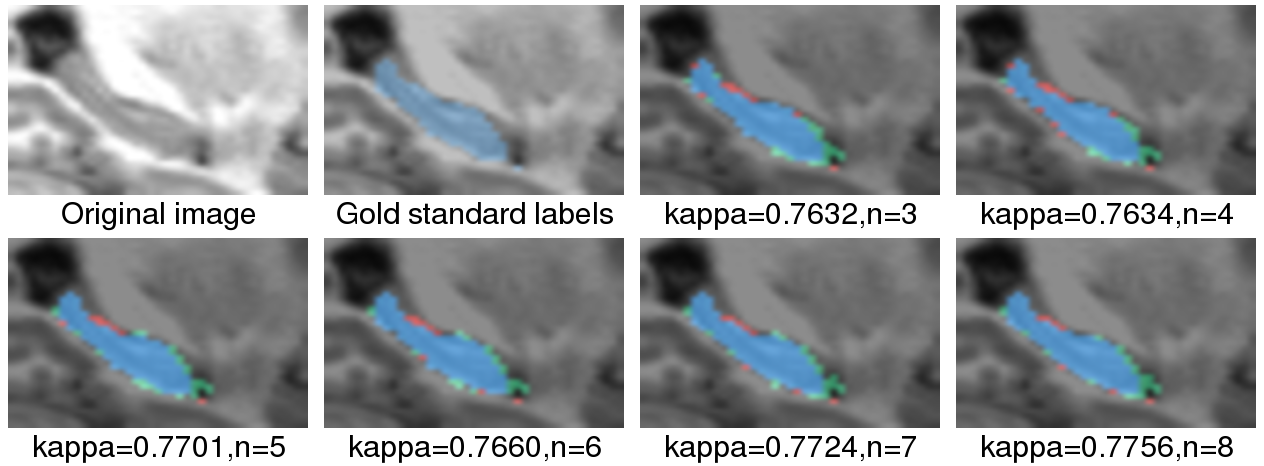
\includegraphics[width=\textwidth]{montage.png}
\end{minipage}
\caption{{\em Sample MAGeT Brain segmentations.} Segmentations of a single
subject are shown when 3 atlases are used, with cross-correlation label
fusion. Blue represents agreement between the gold-standard and MAGeT
Brain.  Red indicates voxels labeled only by the gold-standard, and green
indicates voxels labeled only by MAGeT Brain. Note improved accuracy as the
number of templates is increased.} 
\label{montage}
\end{figure}

In Fig. \ref{results} we compare the performance of the MAGeT Brain method
across all validations (i.e. a combination of all atlases and template
selections) against the multi-atlas method and the naive approach.
Regardless of the number of atlases and templates used in a particular
segmentation we see a marked increase in segmentation accuracy over the
average naive segmentation (the average Kappa of all segmentations derived
from all pairwise registrations in the IBSR dataset).  Clearly, including
more input atlases increases segmentation accuracy.  Surprisingly,
increasing the number of labels in the label fusion step through
cross-correlation based voting, does little to improve segmentation
accuracy (except for in the cases where 3 and 4 atlases are used).
Finally, the best-case MAGeT Brain performance scenario is when 8 atlases
are used.  While this does not reach the accuracy of the multi-atlas
segmentation, there is only a 1.9\% difference in the average Kappa values
($0.775$ for MAGeT Brain with 8 atlases and $0.790$ for multi-atlas after
selecting the top 14 templates).  {SOMETHING IN HERE AS AN EASY WAY TO BOOST ACCURACY FROM THE "ATLAS BASED CASE WOULD BE GOOD TOO}



\begin{figure}
\begin{minipage}[b]{1.0\linewidth}
  \centering
  %\includegraphics[width=\textwidth]{results}
\includegraphics{paper-001}
\end{minipage}
\caption{{\em Performance of MAGeT Brain across all validations compared to
mean naive segmentation, and mean multi-atlas with cross-correlation voting.}
Multi-atlas and naive segmentations procedures provide upper and lower bounds
(respectively) for accuracy.  Note that improved segmentation accuracy is
achieved through increasing the number of input atlases.}
\label{results}
\end{figure}

\section{Discussion}

In this paper, we have demonstrated that accurate segmentations can be
achieved by simply automatically deriving a template library from a small
set of input atlases.  MAGeT Brain segmentations were compared to both
naive segmentations and multi-atlas segmentations with cross-correlation
voting.  In \cite{Lotjonen2010}, the authors report a Kappa of 0.814 on
hippocampal segmentation in the IBSR dataset using a multi-atlas approach
where atlas selection is based on the similarity between atlas and
unlabeled subject after nonlinear registration, and using STAPLE
\cite{Warfield2004} for label fusion.  We demonstrated that the trade off
in accuracy over a multi-atlas segmentation using the entire IBSR manually
segmented library is only on average 1.9\%, using only 8 randomly chosen
atlases.  Discrepancies between our results and the above results may be
due to choice of registration algorithm, regularization parameters, or
similarity metric for label fusion.  Performance may also be affected by
the variability in the IBSR data set (as previously noted by
\cite{Klein2009}).  Future work from our group will attempt to address some
of these issues.

\todo{discuss CC voting and why accuracy is monotonically increasing...
wouldn't we expect an increase and then decrease?}

\bibliographystyle{IEEEbib}
\bibliography{references}
\end{document}
